\chapter*{Сборка проекта}
\addcontentsline{toc}{chapter}{Сборка проекта}

Для сборки проекта необходимо было написать конфигурационный файл. В конфигурационом файле указывается основная информация для работы компилятора v++:

\begin{enumerate}
	\item Количество и условные имена экземпляров ядер.
	\item Тактовая частота работы ядра.
	\item Для каждого ядра: выбор области SLR (SLR[0..2]), выбор DDR (DDR[0..3]) памяти, выбор высокопроизводительной памяти PLRAM( PLRAM[0,1,2]).
	\item Параметры синтеза и оптимизации проекта.
\end{enumerate}

На рисунке \ref{png:configure} представлен конфигурационный файл для сборки проекта.

\begin{figure}[H]
	\captionsetup{justification=centering}
	\centering{
		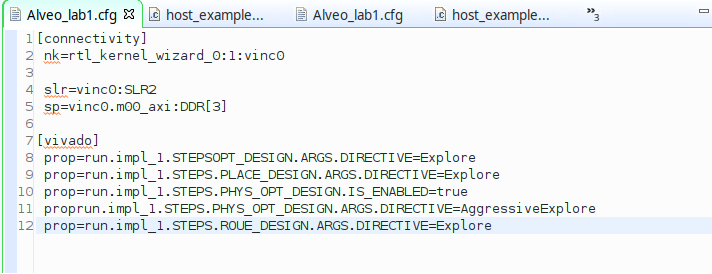
\includegraphics[scale=1]{images/cfg_file}
		\caption{Конфигурационный файл}
		\label{png:configure}
	}
\end{figure}
Содержимое файлов v++*.log и *.xclbin.info. приведено в приложениях.

\chapter*{Тестирование}
\addcontentsline{toc}{chapter}{Тестирование}

Для того, чтобы запустить тесты, необходимо изменить условие проверки в автоматически созданном программном модуле host\_example.cpp.

Часть кода модуля host\_example.cpp приведена на рисунке \ref{png:new_host}. Было изменено условие проверки, на проверку, соответствующую моему варианту.

\begin{figure}[H]
	\captionsetup{justification=centering}
	\centering{
		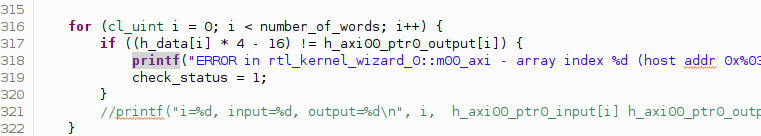
\includegraphics[scale=1]{images/new_code}
		\caption{Фрагмент кода host\_example.cpp}
		\label{png:new_host}
	}
\end{figure}

Тесты запускались с помощью команды Run->Run Configurations с настройкой параметров согласно условию лабораторной работы. По результатам на рисунке \ref{png:test} можно увидеть, что все тесты выполнены успешно.

\begin{figure}[H]
	\captionsetup{justification=centering}
	\centering{
		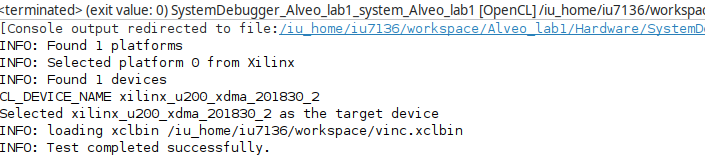
\includegraphics[scale=1]{images/test}
		\caption{Выполнение тестов}
		\label{png:test}
	}
\end{figure}

